\section{Assembly Process (Jakub Jędrzejczyk)}

% Figures \ref{fig:FinalAssembly000-010}, \ref{fig:FinalAssembly020-030}, \ref{fig:FinalAssembly040-051}, \ref{fig:FinalAssembly060-070}, \ref{fig:FinalAssembly080-090}, \ref{fig:FinalAssembly100-110}, \ref{fig:FinalAssembly120-130}, \ref{fig:FinalAssembly140-150}, \ref{fig:FinalAssembly160-170} below is a set of comic-style images illustrating the process of assembling a PC using the developed VR application.

Figures \ref{fig:FinalAssembly000}, \ref{fig:FinalAssembly010}, \ref{fig:FinalAssembly020}, \ref{fig:FinalAssembly030}, \ref{fig:FinalAssembly040}, \ref{fig:FinalAssembly051}, \ref{fig:FinalAssembly060}, \ref{fig:FinalAssembly070}, \ref{fig:FinalAssembly080}, \ref{fig:FinalAssembly090}, \ref{fig:FinalAssembly100}, \ref{fig:FinalAssembly110}, \ref{fig:FinalAssembly120}, \ref{fig:FinalAssembly130}, \ref{fig:FinalAssembly140}, \ref{fig:FinalAssembly150}, \ref{fig:FinalAssembly160}, \ref{fig:FinalAssembly170} below are a set of comic-style images illustrating the process of assembling a PC using the developed VR application.

% \begin{figure}[H]
% 	\centering
% 	\subfigure[]{
% 		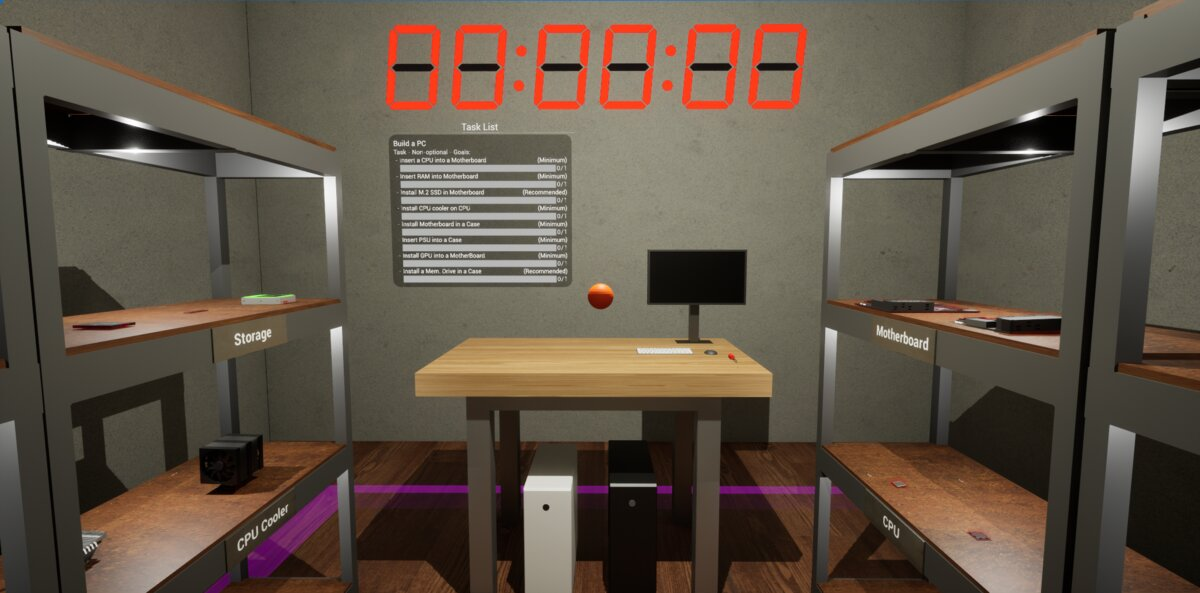
\includegraphics[width=0.48\textwidth]{Images/FinalAssembly000-optimized-hard.jpg}
% 		\label{fig:FinalAssembly000}
% 	}%
% 	\hfil
% 	\subfigure[]{
% 		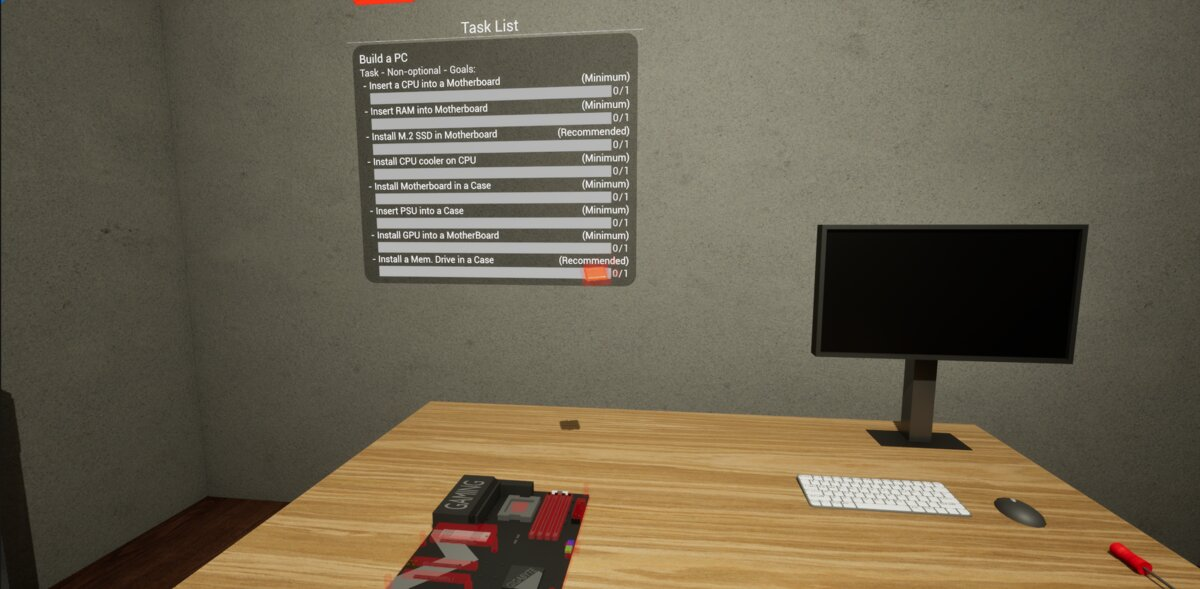
\includegraphics[width=0.48\textwidth]{Images/FinalAssembly010-optimized-hard.jpg}
% 		\label{fig:FinalAssembly010}
% 	}
% 	\caption{Beginning of the assembly process: (a) Starting of the assembly process, right after launching the application. (b) The user moved the motherboard to the table, and has picked up a compatible CPU.}
%     \label{fig:FinalAssembly000-010}
% \end{figure}

\begin{figure}[H]
	\centering
	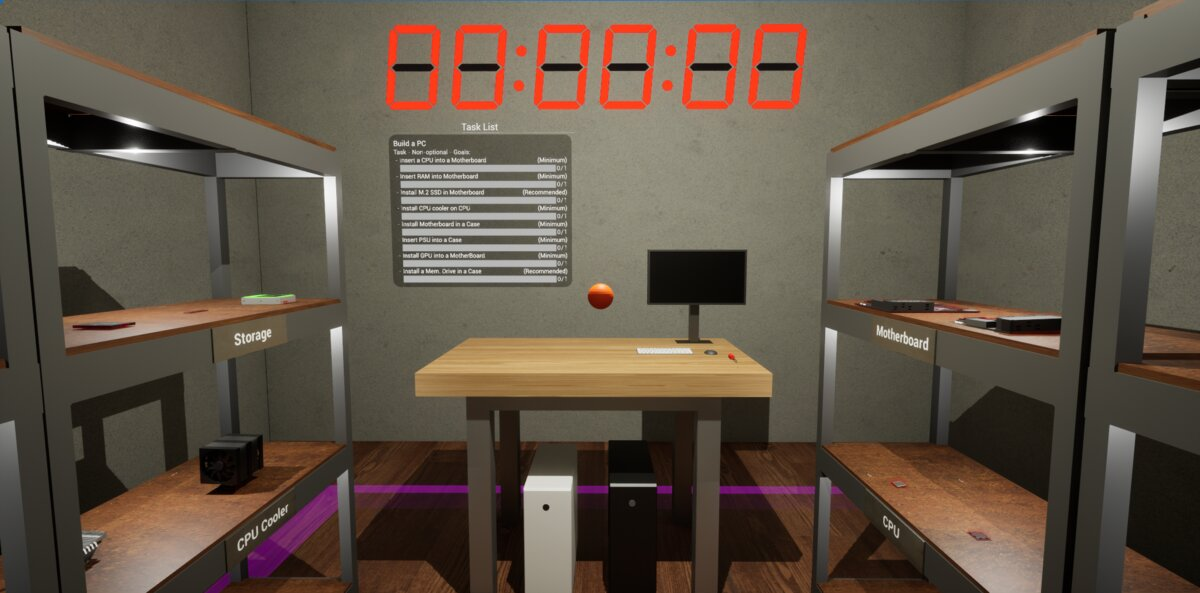
\includegraphics[width=1.0\textwidth]{Images/FinalAssembly000-optimized-hard.jpg}
	\caption{Starting of the assembly process, right after launching the application.}
    \label{fig:FinalAssembly000}
\end{figure}

\begin{figure}[H]
	\centering
	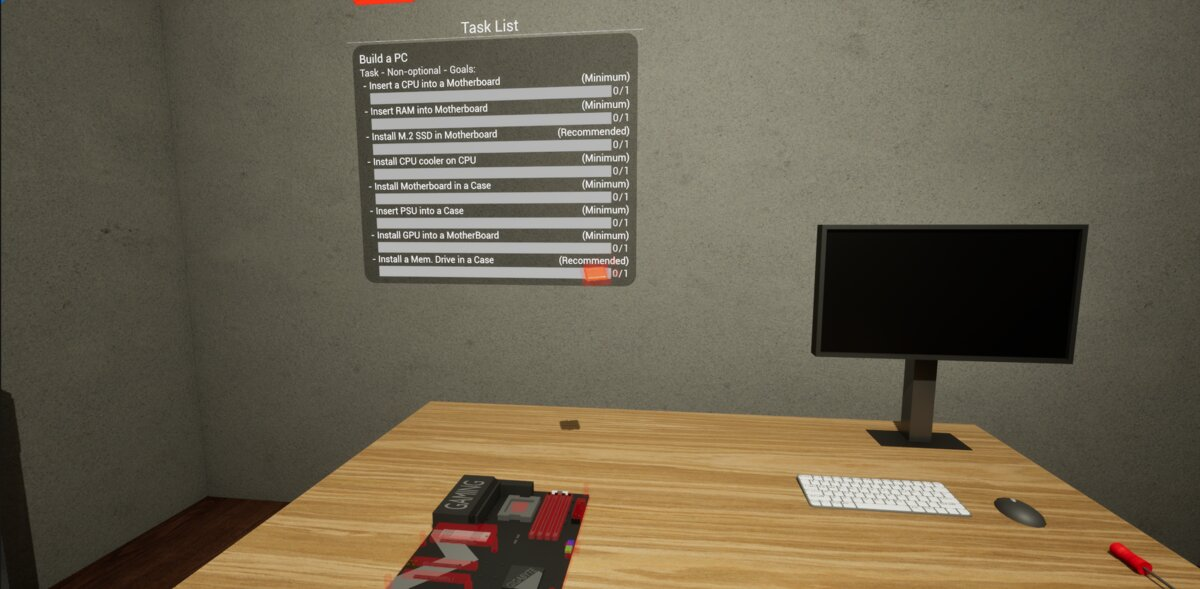
\includegraphics[width=1.0\textwidth]{Images/FinalAssembly010-optimized-hard.jpg}
	\caption{The user moved the motherboard to the table, and has picked up a compatible CPU.}
	\label{fig:FinalAssembly010}
\end{figure}

% \begin{figure}[H]
% 	\centering
% 	\subfigure[]{
% 		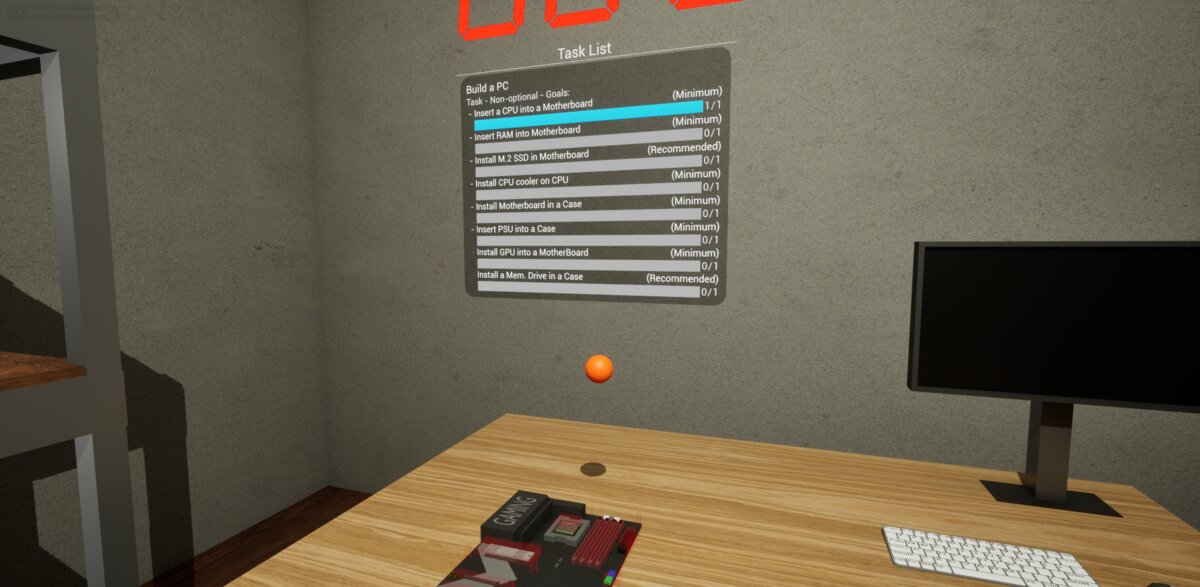
\includegraphics[width=0.48\textwidth]{Images/FinalAssembly020-optimized-hard.jpg}
% 		\label{fig:FinalAssembly020}
% 	}%
% 	\hfil
% 	\subfigure[]{
% 		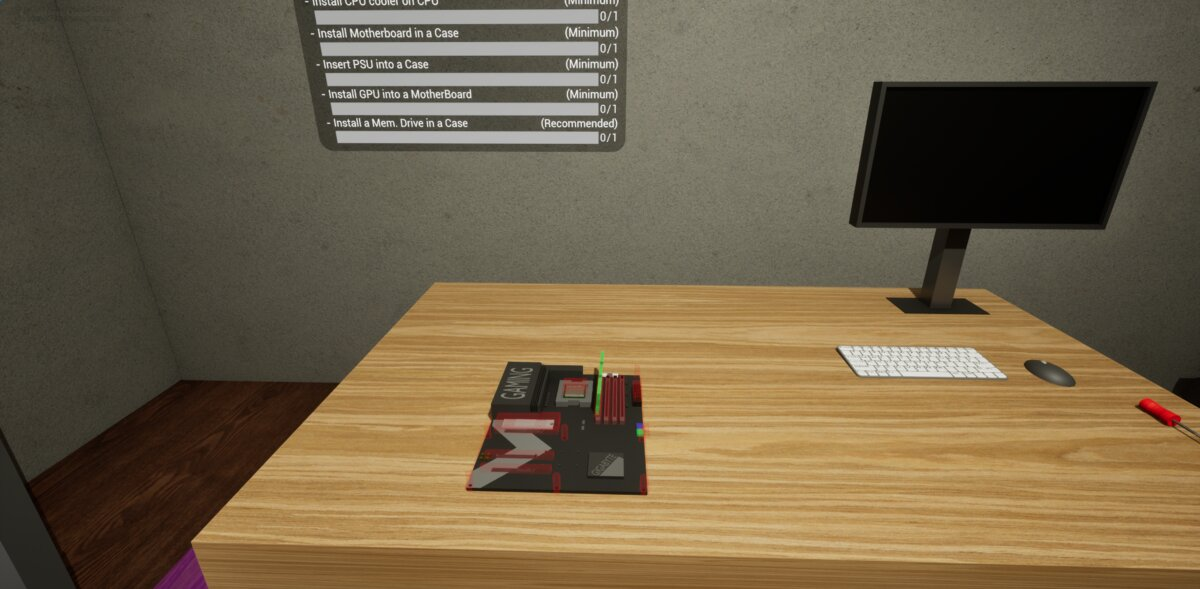
\includegraphics[width=0.48\textwidth]{Images/FinalAssembly030-optimized-hard.jpg}
% 		\label{fig:FinalAssembly030}
% 	}
% 	\caption{Connecting components to the motherboard: (a) As a result of the CPU installation, the task list was updated to reflect the user's progress. (b) The user has picked up a RAM module, and is lining it up with the motherboard's RAM slot.}
%     \label{fig:FinalAssembly020-030}
% \end{figure}

\begin{figure}[H]
	\centering
	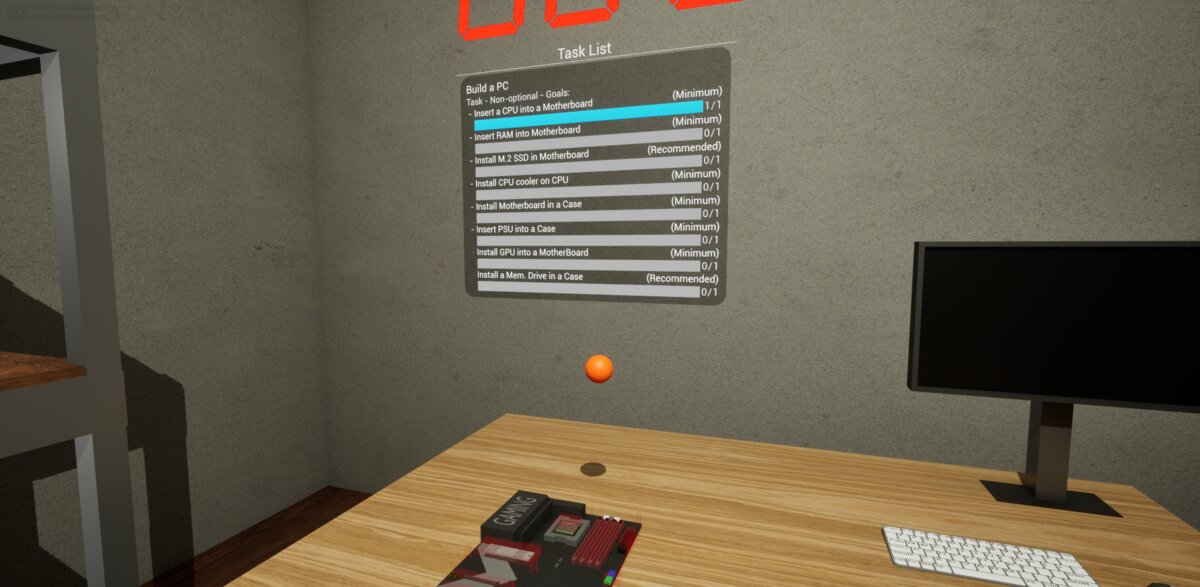
\includegraphics[width=0.973\textwidth]{Images/FinalAssembly020-optimized-hard.jpg}
	\caption{As a result of the CPU installation, the task list was updated to reflect the user's progress.}
	\label{fig:FinalAssembly020}
\end{figure}

\begin{figure}[H]
	\centering
	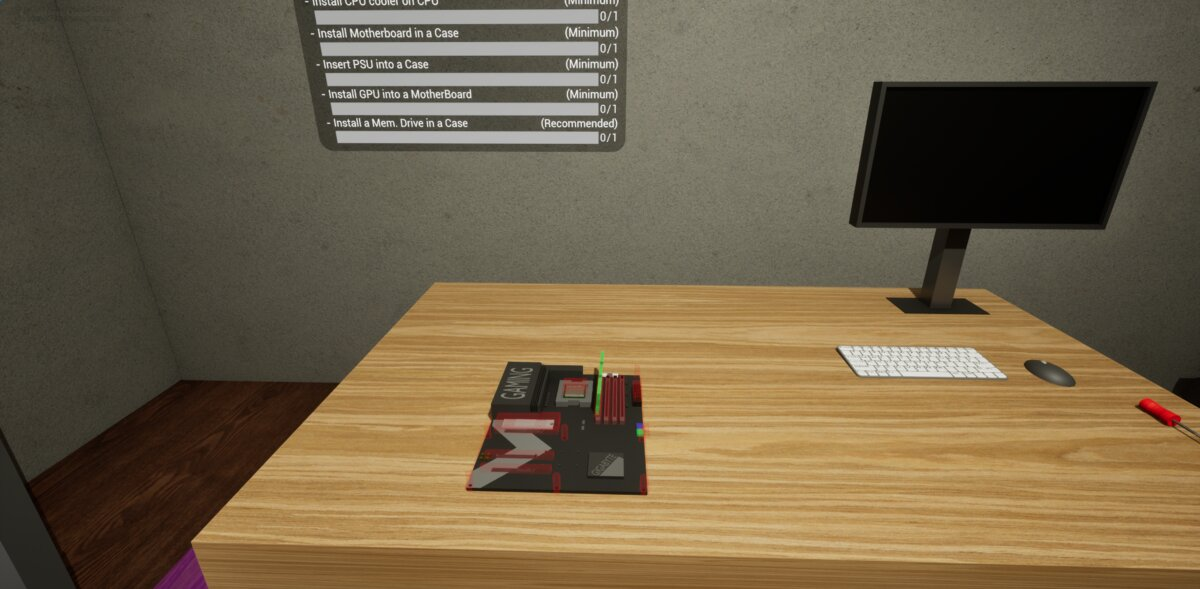
\includegraphics[width=0.973\textwidth]{Images/FinalAssembly030-optimized-hard.jpg}
	\caption{The user has picked up a RAM module, and is lining it up with the motherboard's RAM slot.}
	\label{fig:FinalAssembly030}
\end{figure}

% \begin{figure}[H]
% 	\centering
% 	\subfigure[]{
% 		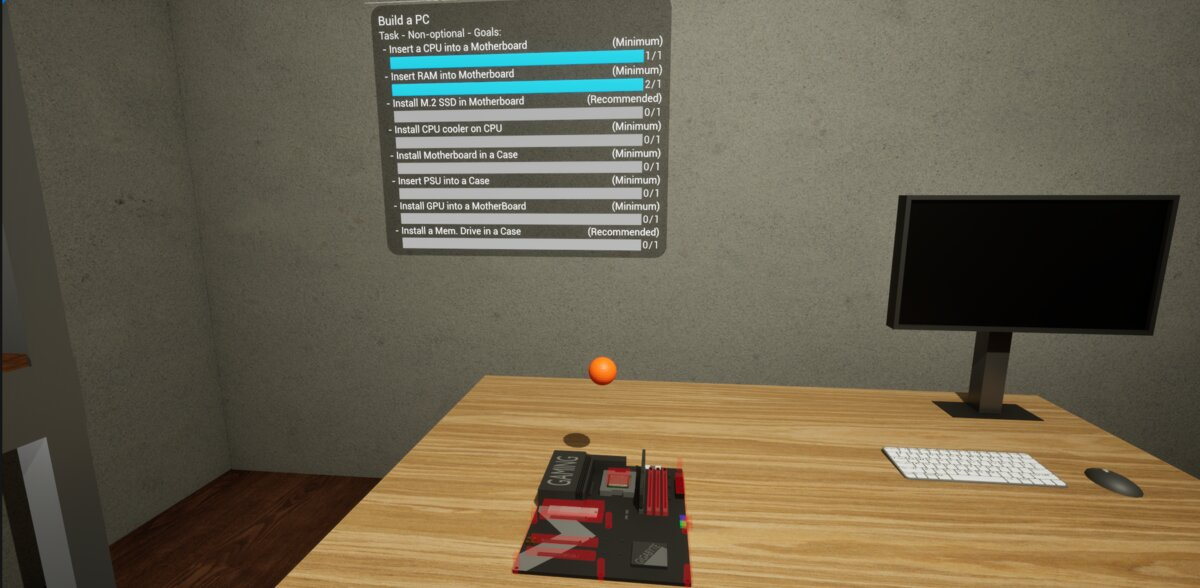
\includegraphics[width=0.48\textwidth]{Images/FinalAssembly040-optimized-hard.jpg}
% 		\label{fig:FinalAssembly040}
% 	}%
% 	\hfil
% 	\subfigure[]{
% 		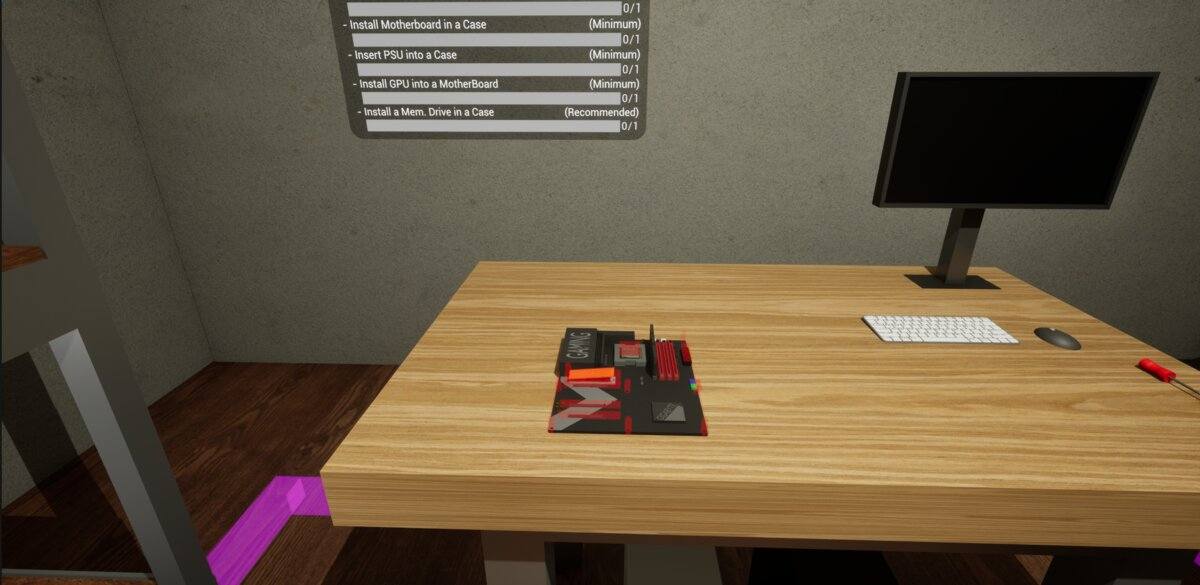
\includegraphics[width=0.48\textwidth]{Images/FinalAssembly051-optimized-hard.jpg}
% 		\label{fig:FinalAssembly051}
% 	}
% 	\caption{Continued work with the motherboard: (a) Once the RAM has been installed, the task list has been updated accordingly. (b) Following the list, the user is attempting to install a drive into the motherboard's M.2 slot, but will need to rotate it first.}
%     \label{fig:FinalAssembly040-051}
% \end{figure}

\begin{figure}[H]
	\centering
	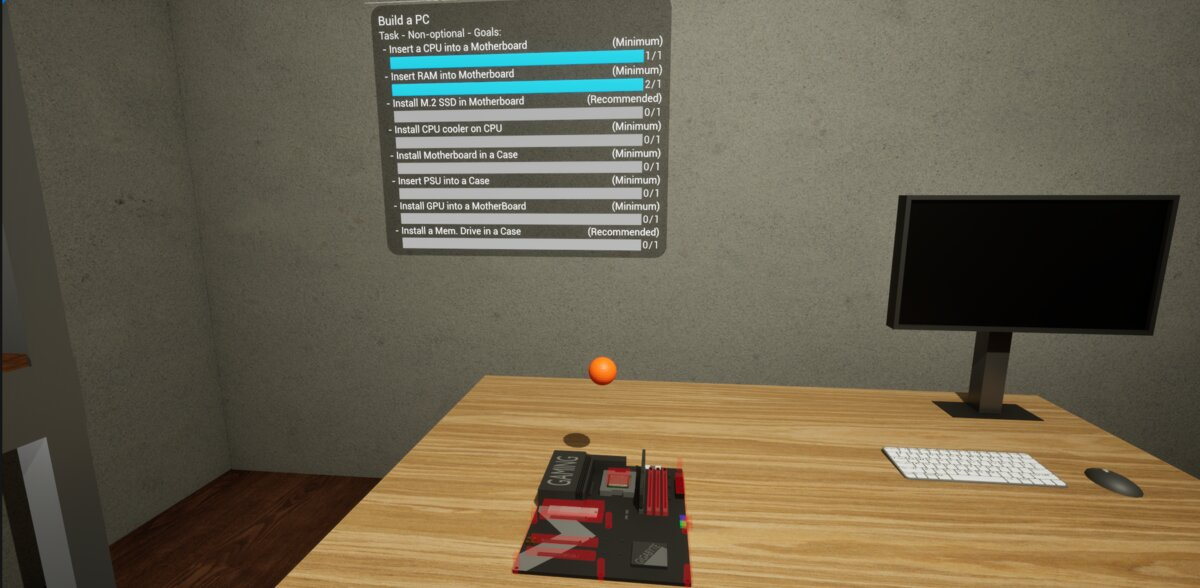
\includegraphics[width=0.973\textwidth]{Images/FinalAssembly040-optimized-hard.jpg}
	\caption{Once the RAM has been installed, the task list has been updated accordingly.}
	\label{fig:FinalAssembly040}
\end{figure}

\begin{figure}[H]
	\centering
	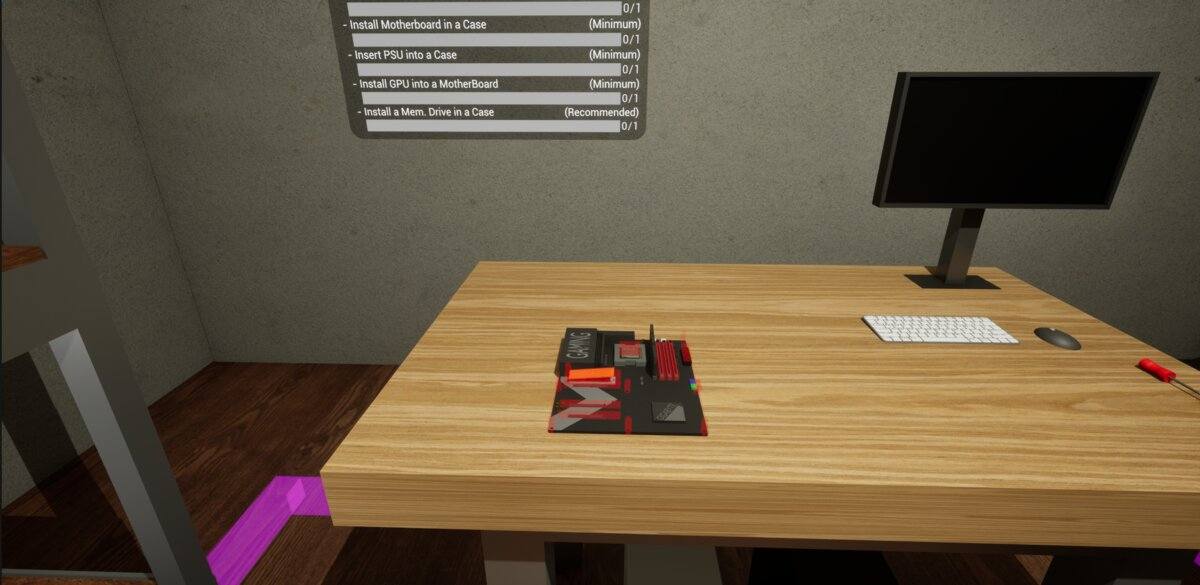
\includegraphics[width=0.932\textwidth]{Images/FinalAssembly051-optimized-hard.jpg}
	\caption{Following the list, the user is attempting to install a drive into the motherboard's M.2 slot, but will need to rotate it first.}
	\label{fig:FinalAssembly051}
\end{figure}

% \begin{figure}[H]
% 	\centering
% 	\subfigure[]{
% 		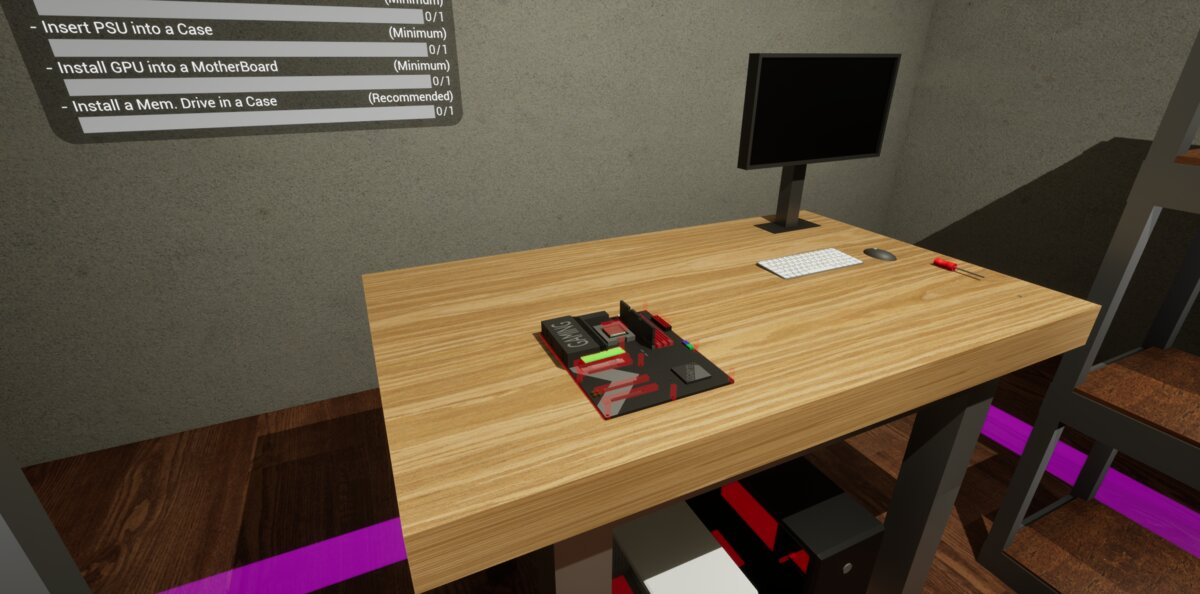
\includegraphics[width=0.48\textwidth]{Images/FinalAssembly060-optimized-hard.jpg}
% 		\label{fig:FinalAssembly060}
% 	}%
% 	\hfil
% 	\subfigure[]{
% 		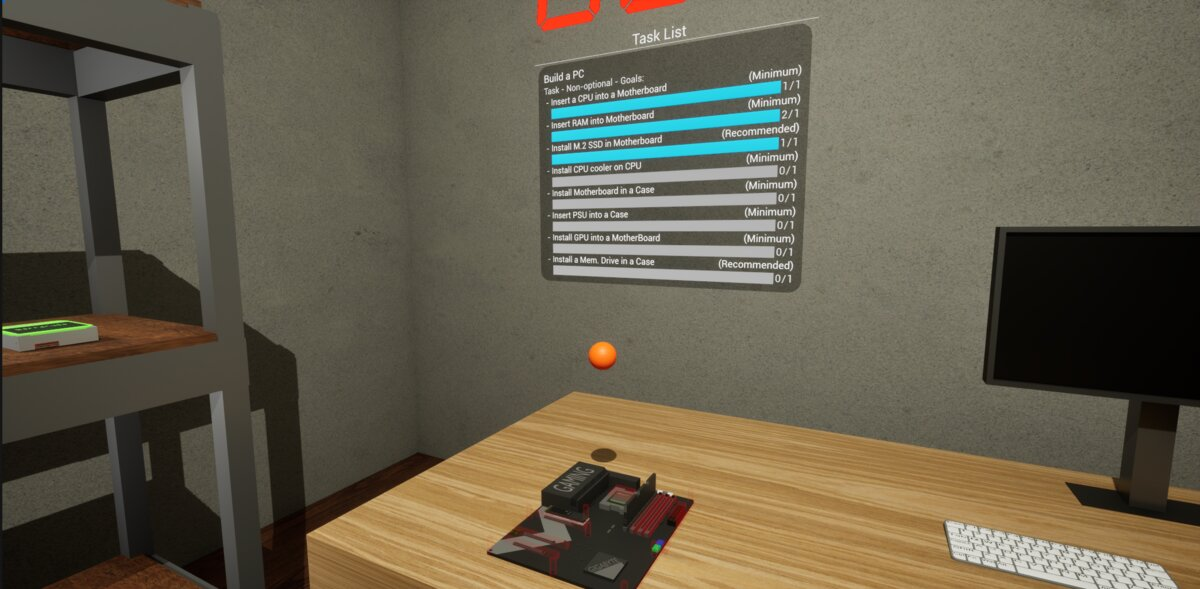
\includegraphics[width=0.48\textwidth]{Images/FinalAssembly070-optimized-hard.jpg}
% 		\label{fig:FinalAssembly070}
% 	}
% 	\caption{Fixing the drive issue: (a) After the drive has been rotated, it can be properly installed. (b) The drive has been successfully installed, and the task list has been updated to reflect the user's progress.}
%     \label{fig:FinalAssembly060-070}
% \end{figure}

\begin{figure}[H]
	\centering
	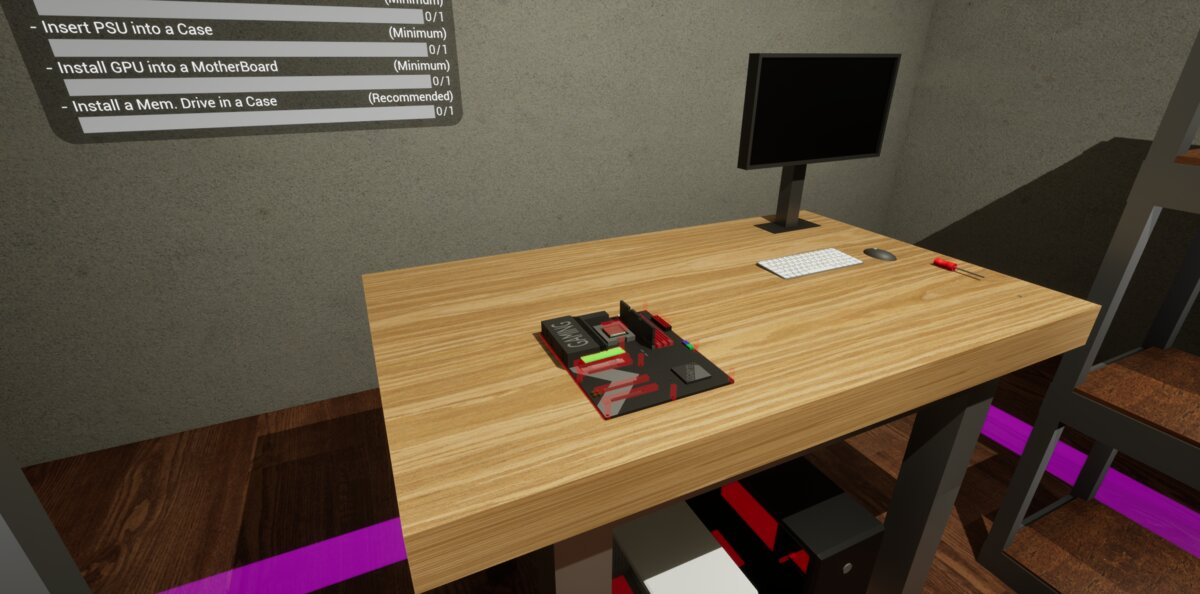
\includegraphics[width=0.932\textwidth]{Images/FinalAssembly060-optimized-hard.jpg}
	\caption{After the drive has been rotated, it can be properly installed.}
	\label{fig:FinalAssembly060}
\end{figure}

\begin{figure}[H]
	\centering
	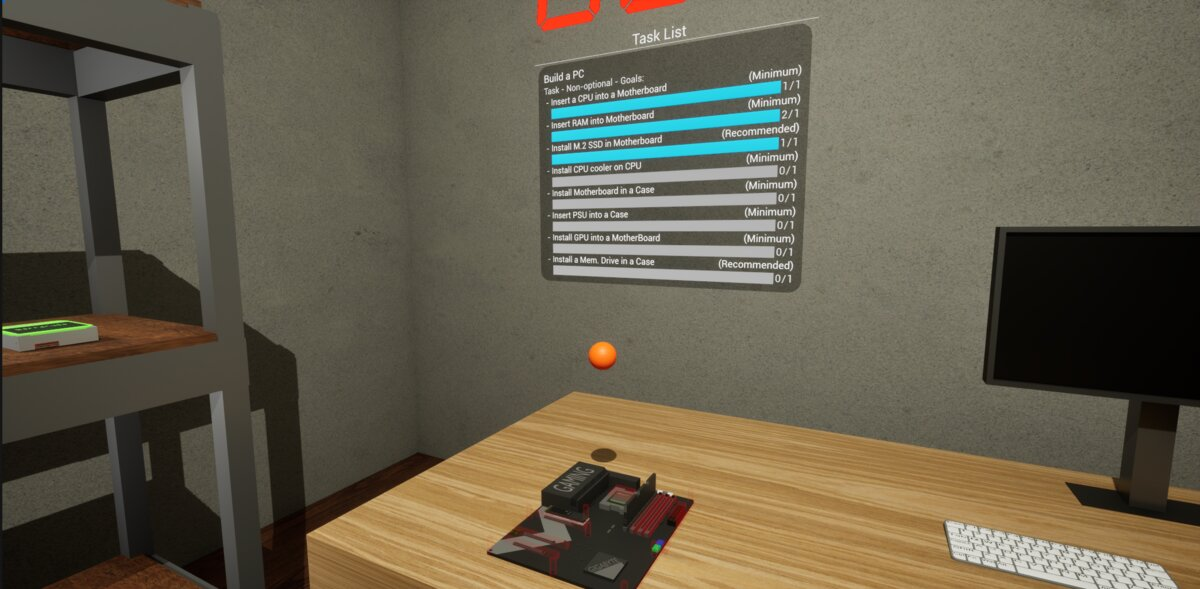
\includegraphics[width=0.932\textwidth]{Images/FinalAssembly070-optimized-hard.jpg}
	\caption{The drive has been successfully installed, and the task list has been updated to reflect the user's progress.}
	\label{fig:FinalAssembly070}
\end{figure}

% \begin{figure}[H]
% 	\centering
% 	\subfigure[]{
% 		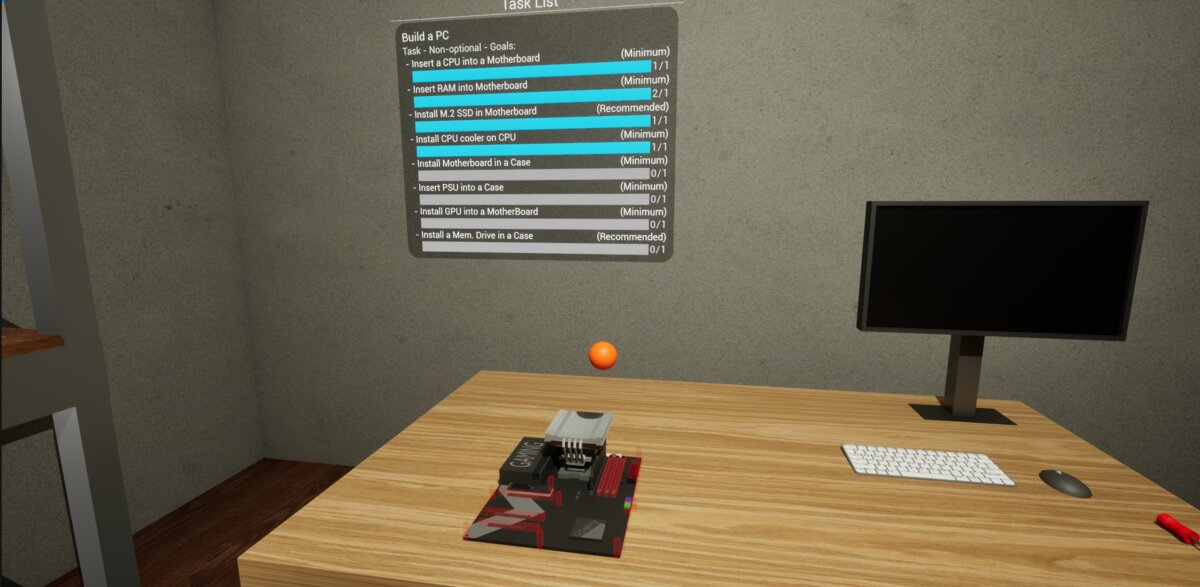
\includegraphics[width=0.48\textwidth]{Images/FinalAssembly080-optimized-hard.jpg}
% 		\label{fig:FinalAssembly080}
% 	}%
% 	\hfil
% 	\subfigure[]{
% 		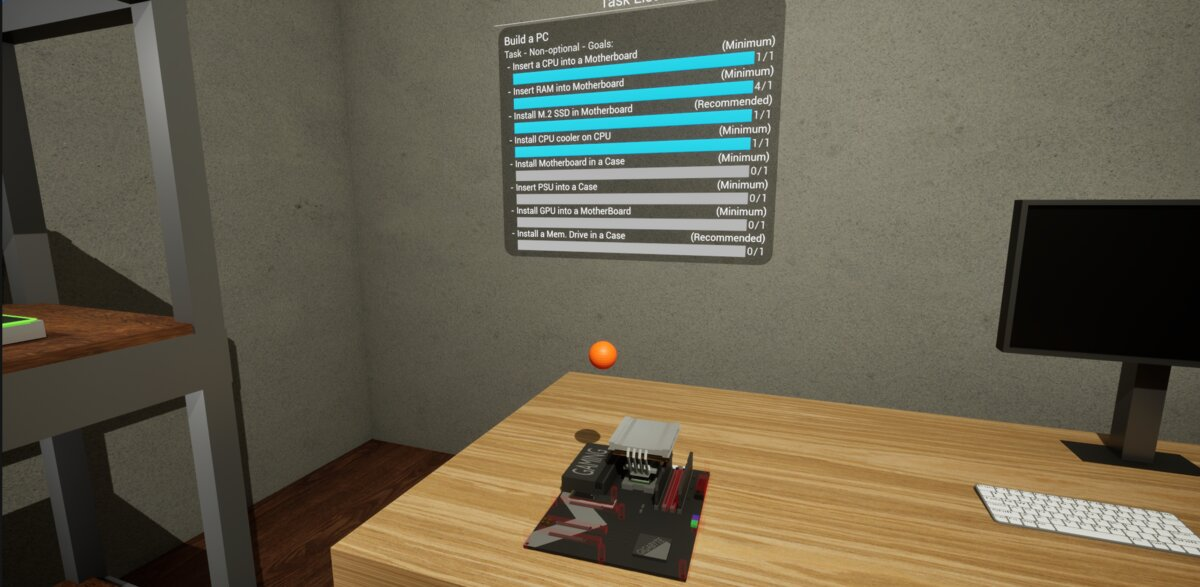
\includegraphics[width=0.48\textwidth]{Images/FinalAssembly090-optimized-hard.jpg}
% 		\label{fig:FinalAssembly090}
% 	}
% 	\caption{Finishing the motherboard assembly: (a) A cooler has been installed on the CPU. (b) The user has decided to add another RAM stick, this time on the far right of the motherboard.}
%     \label{fig:FinalAssembly080-090}
% \end{figure}

\begin{figure}[H]
	\centering
	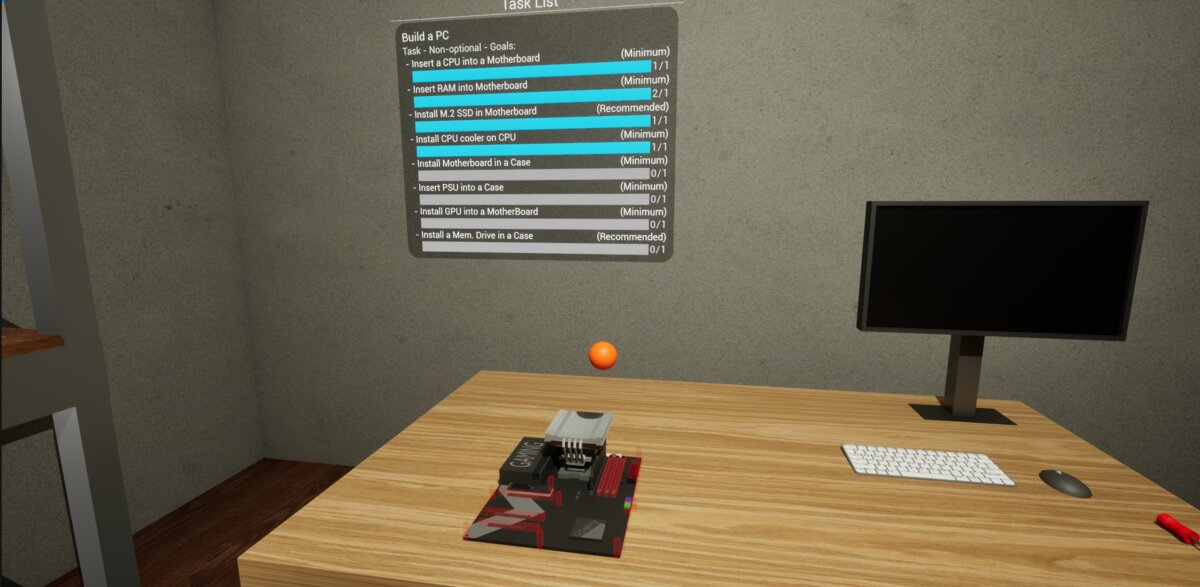
\includegraphics[width=0.973\textwidth]{Images/FinalAssembly080-optimized-hard.jpg}
	\caption{A cooler has been installed on the CPU.}
	\label{fig:FinalAssembly080}
\end{figure}

\begin{figure}[H]
	\centering
	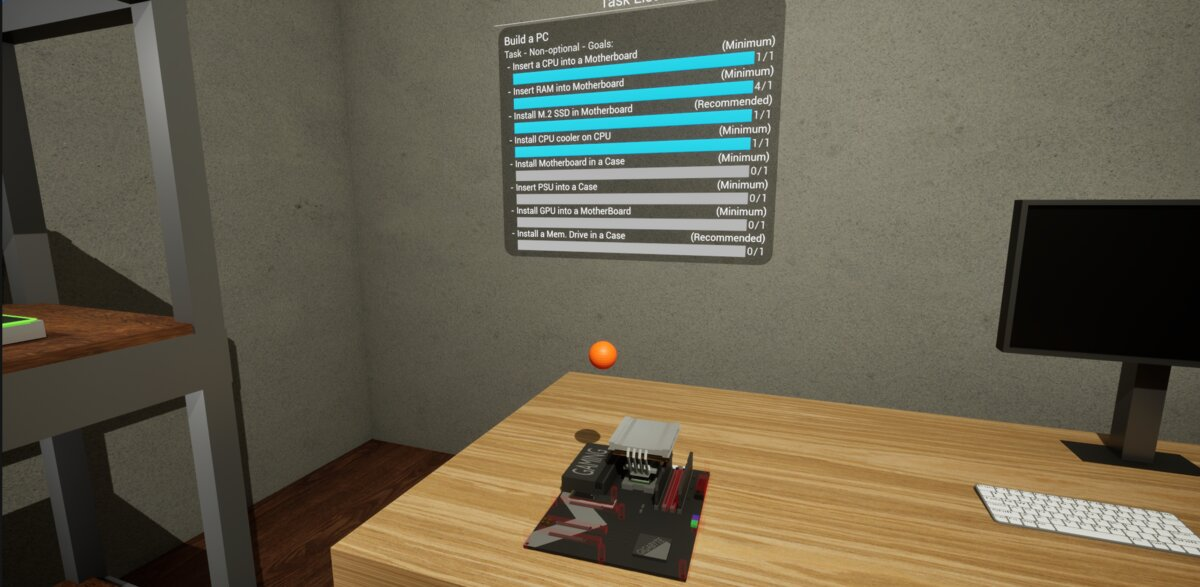
\includegraphics[width=0.973\textwidth]{Images/FinalAssembly090-optimized-hard.jpg}
	\caption{The user has decided to add another RAM stick, this time on the far right of the motherboard.}
	\label{fig:FinalAssembly090}
\end{figure}

% \begin{figure}[H]
% 	\centering
% 	\subfigure[]{
% 		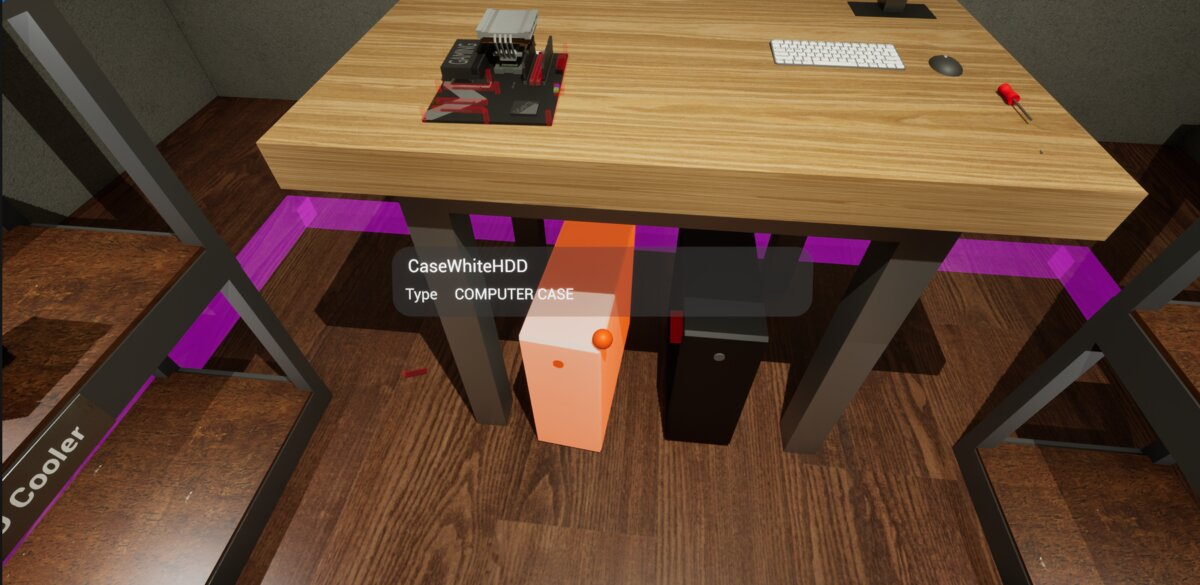
\includegraphics[width=0.45\textwidth]{Images/FinalAssembly100-optimized-hard.jpg}
% 		\label{fig:FinalAssembly100}
% 	}%
% 	\hfil
% 	\subfigure[]{
% 		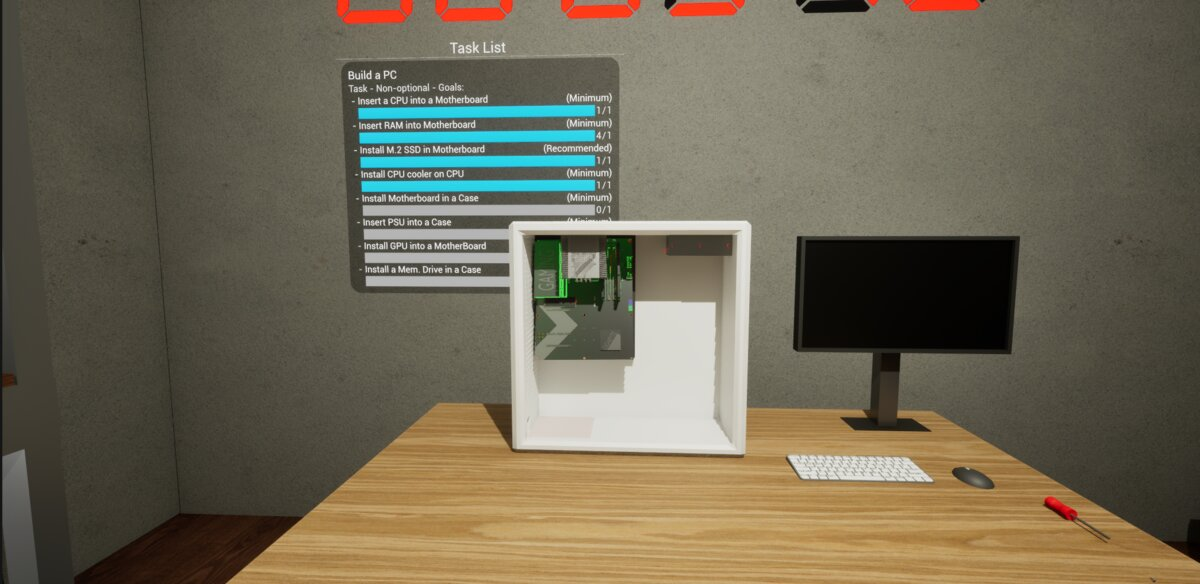
\includegraphics[width=0.45\textwidth]{Images/FinalAssembly110-optimized-hard.jpg}
% 		\label{fig:FinalAssembly110}
% 	}
% 	\caption{Adding a case to the build: (a) The user picks the white case, which can have a 3.5" hard drive installed in it. (b) The case has been placed on the table, and the user is attempting to put the motherboard inside it.}
%     \label{fig:FinalAssembly100-110}
% \end{figure}

\begin{figure}[H]
	\centering
	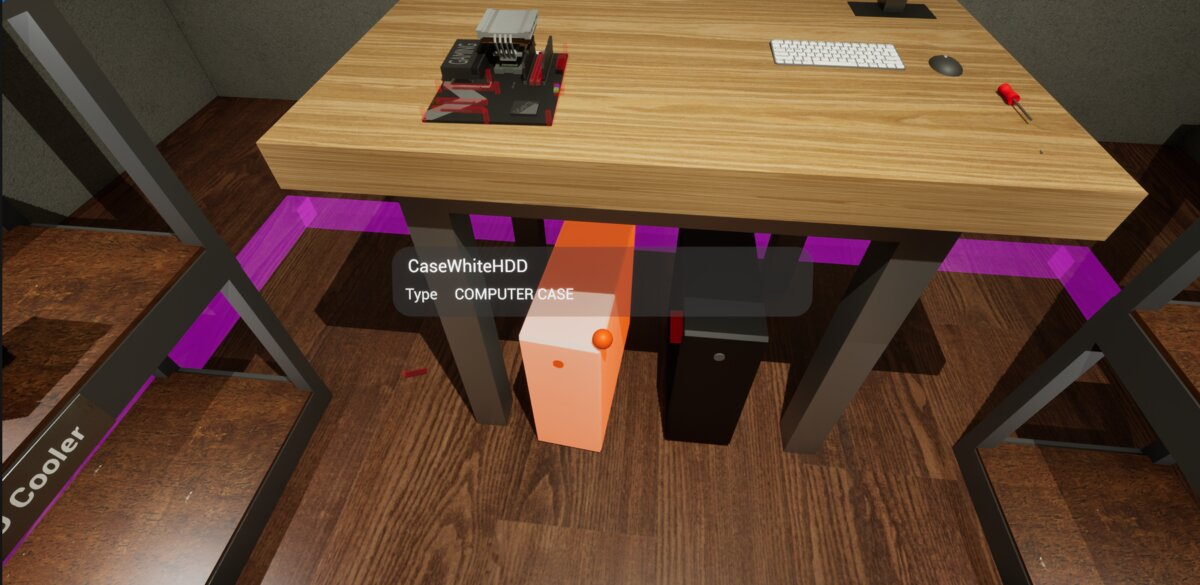
\includegraphics[width=0.973\textwidth]{Images/FinalAssembly100-optimized-hard.jpg}
	\caption{The user picks the white case, which can have a 3.5" hard drive installed in it.}
	\label{fig:FinalAssembly100}
\end{figure}

\begin{figure}[H]
	\centering
	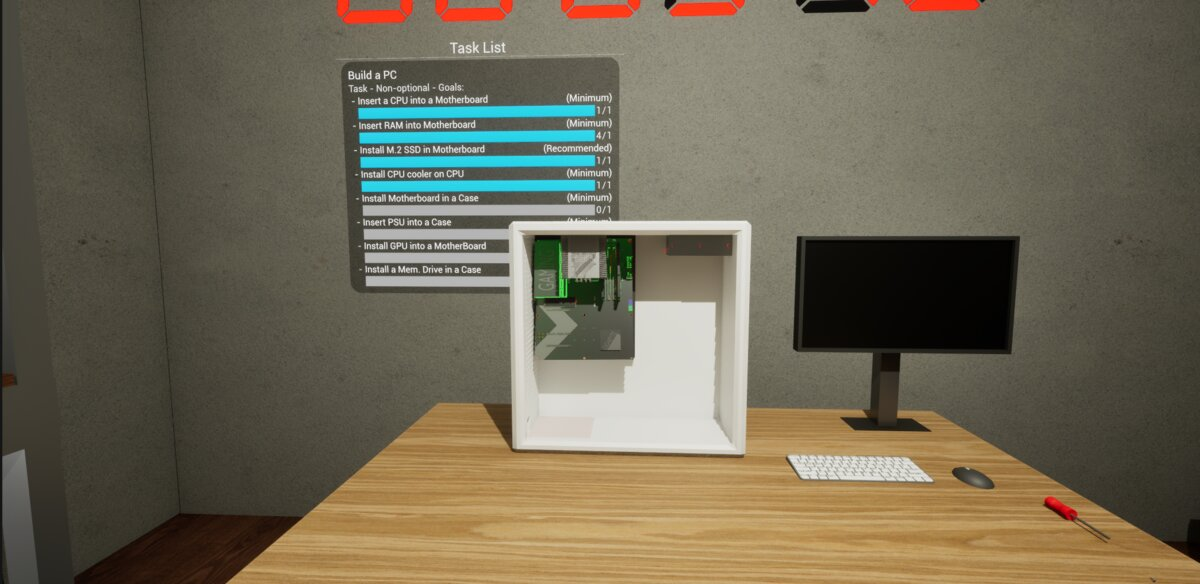
\includegraphics[width=0.961\textwidth]{Images/FinalAssembly110-optimized-hard.jpg}
	\caption{The case has been placed on the table, and the user is attempting to put the motherboard inside it.}
	\label{fig:FinalAssembly110}
\end{figure}

% \begin{figure}[H]
% 	\centering
% 	\subfigure[]{
% 		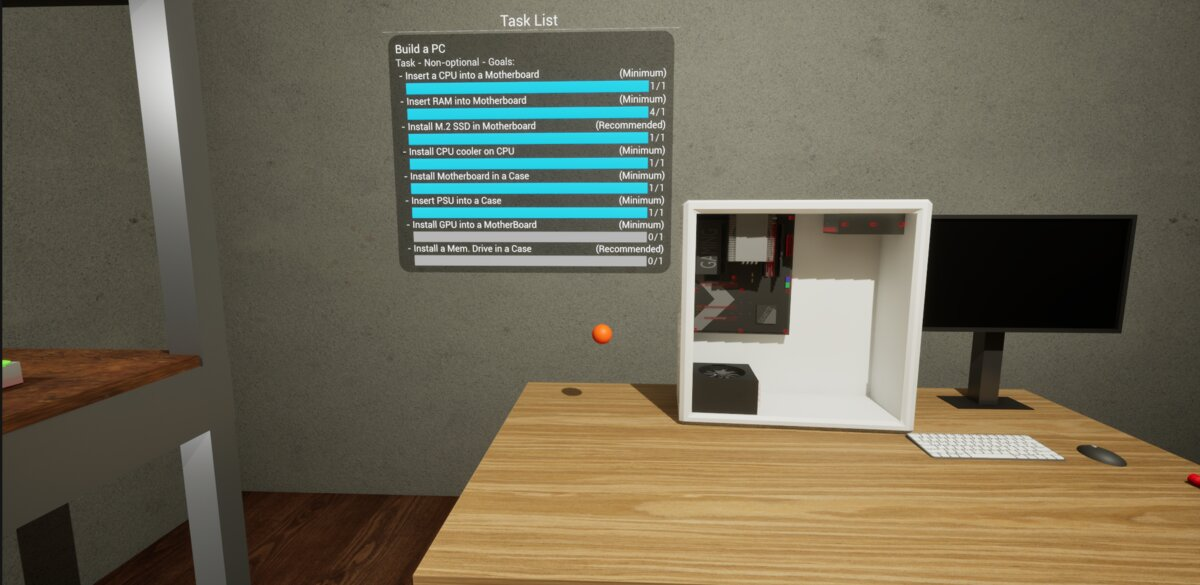
\includegraphics[width=0.45\textwidth]{Images/FinalAssembly120-optimized-hard.jpg}
% 		\label{fig:FinalAssembly120}
% 	}%
% 	\hfil
% 	\subfigure[]{
% 		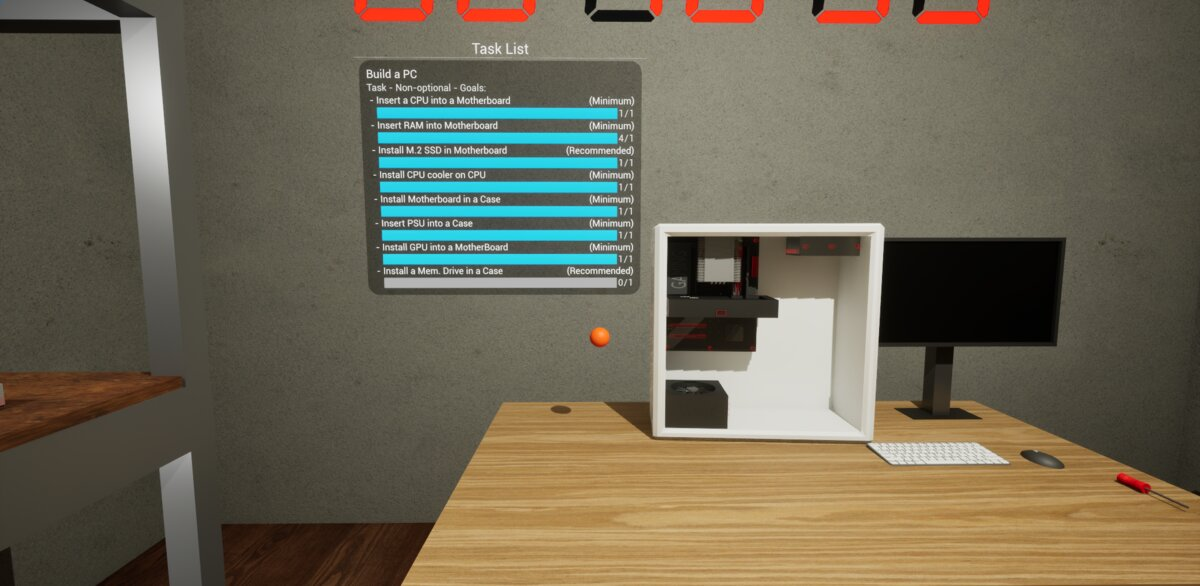
\includegraphics[width=0.45\textwidth]{Images/FinalAssembly130-optimized-hard.jpg}
% 		\label{fig:FinalAssembly130}
% 	}
% 	\caption{Working in the case: (a) A PSU has been placed in the case, which is reflected in the task list. (b) The GPU has been installed in the motherboard's PCIe slot, again reflected in the task list.}
%     \label{fig:FinalAssembly120-130}
% \end{figure}

\begin{figure}[H]
	\centering
	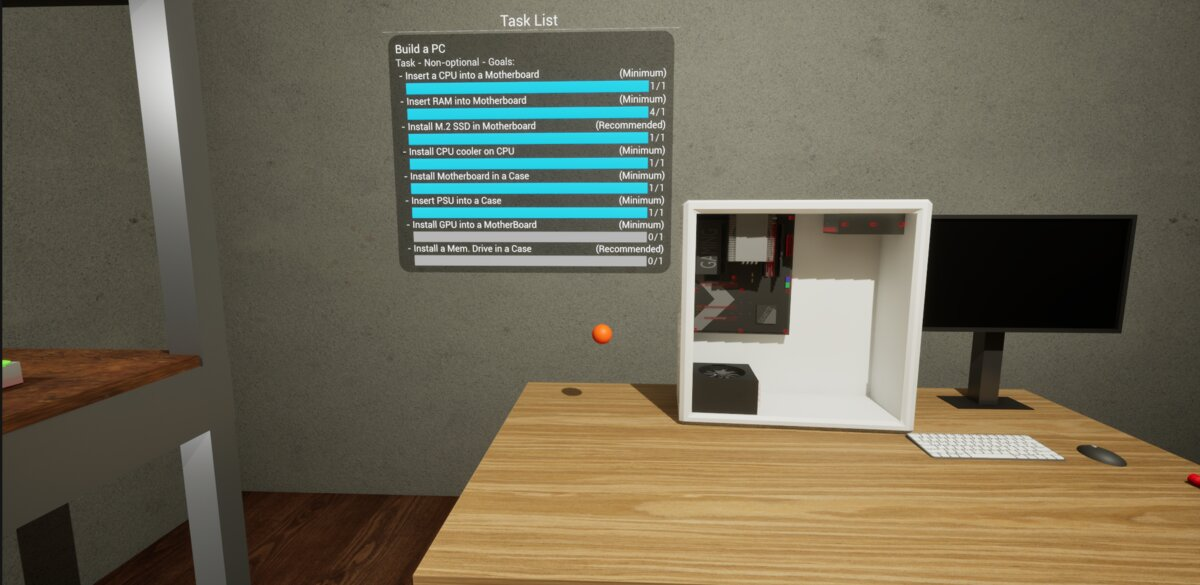
\includegraphics[width=0.961\textwidth]{Images/FinalAssembly120-optimized-hard.jpg}
	\caption{A PSU has been placed in the case, which is reflected in the task list.}
	\label{fig:FinalAssembly120}
\end{figure}

\begin{figure}[H]
	\centering
	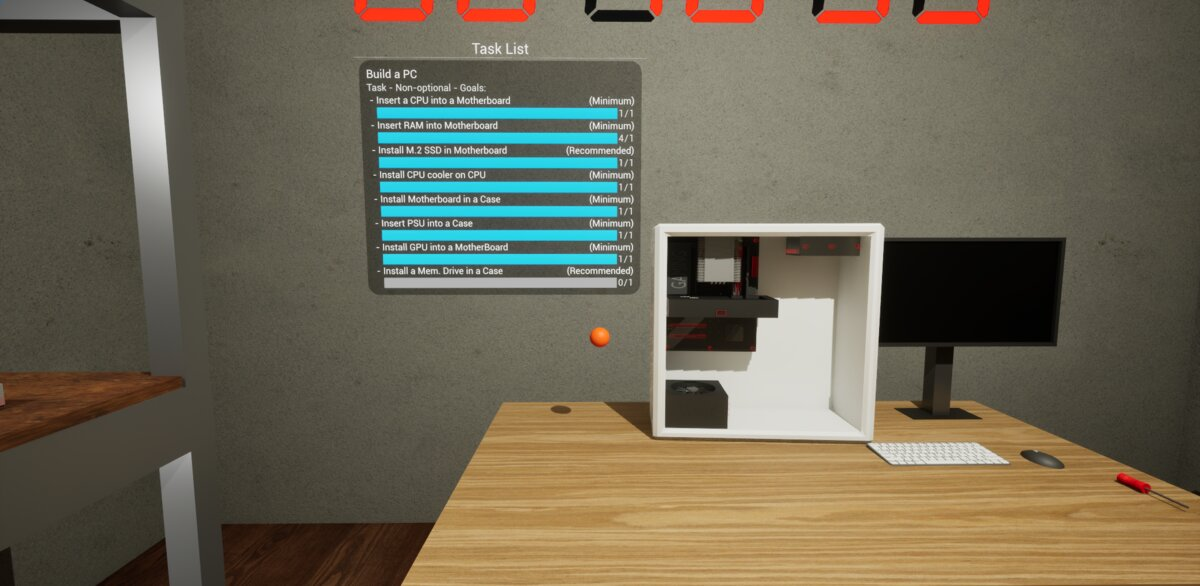
\includegraphics[width=0.961\textwidth]{Images/FinalAssembly130-optimized-hard.jpg}
	\caption{The GPU has been installed in the motherboard's PCIe slot, again reflected in the task list.}
	\label{fig:FinalAssembly130}
\end{figure}

% \begin{figure}[H]
% 	\centering
% 	\subfigure[]{
% 		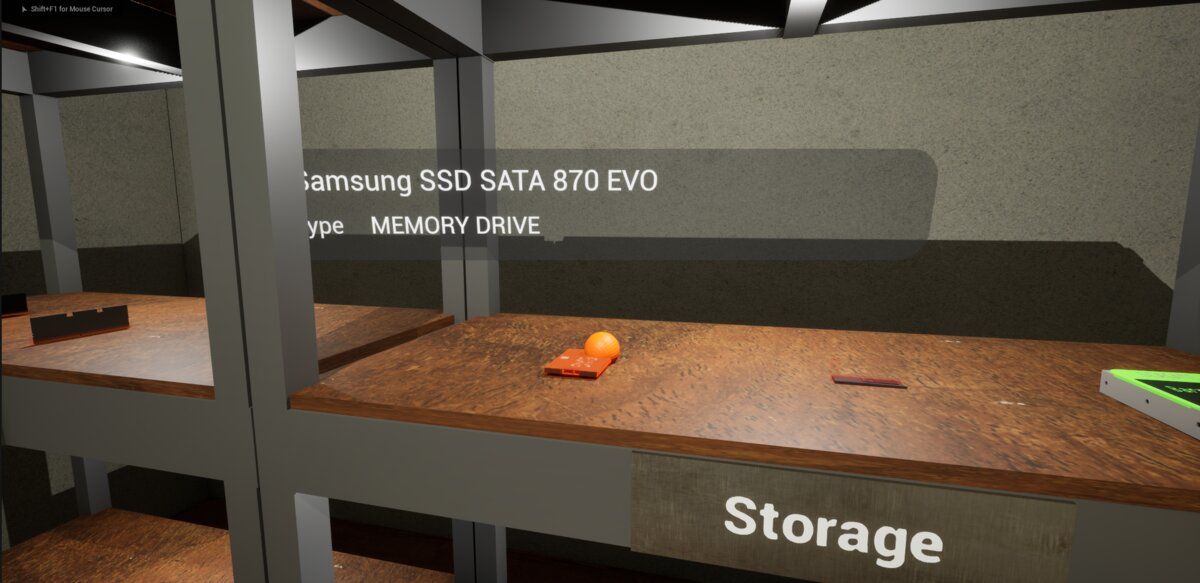
\includegraphics[width=0.45\textwidth]{Images/FinalAssembly140-optimized-hard.jpg}
% 		\label{fig:FinalAssembly140}
% 	}%
% 	\hfil
% 	\subfigure[]{
% 		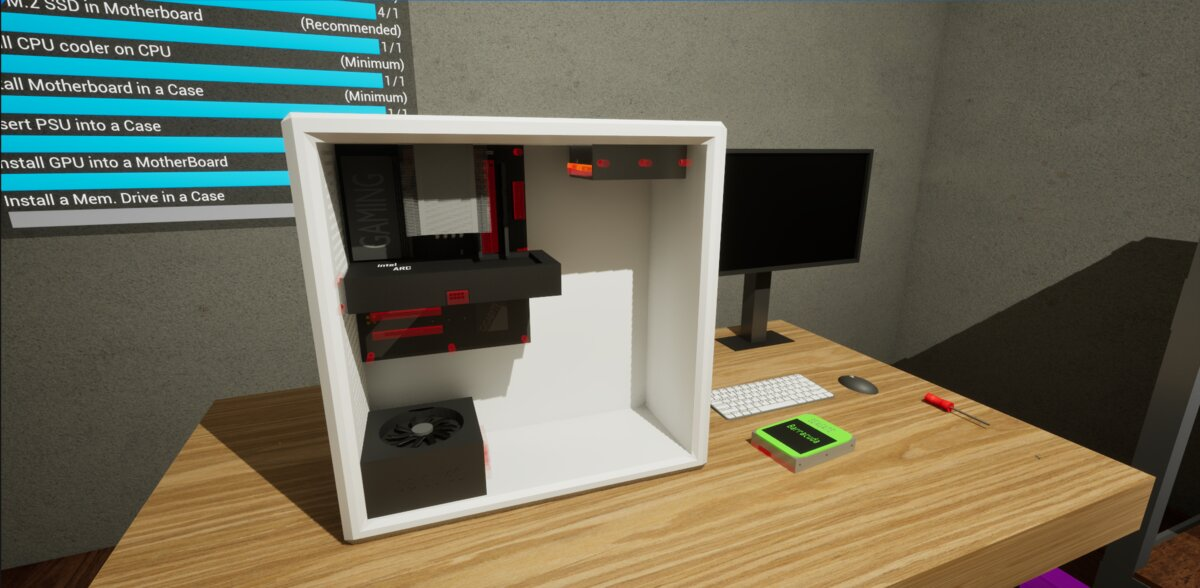
\includegraphics[width=0.45\textwidth]{Images/FinalAssembly150-optimized-hard.jpg}
% 		\label{fig:FinalAssembly150}
% 	}
% 	\caption{Attempting to install an SSD: (a) Despite knowing the case is not compatible, the user picks an SSD to install in the case. (b) Despite lining it up correctly, the SSD does not highlight as possible to be connected with the case, indicating incompatibility.}
%     \label{fig:FinalAssembly140-150}
% \end{figure}

\begin{figure}
	\centering
	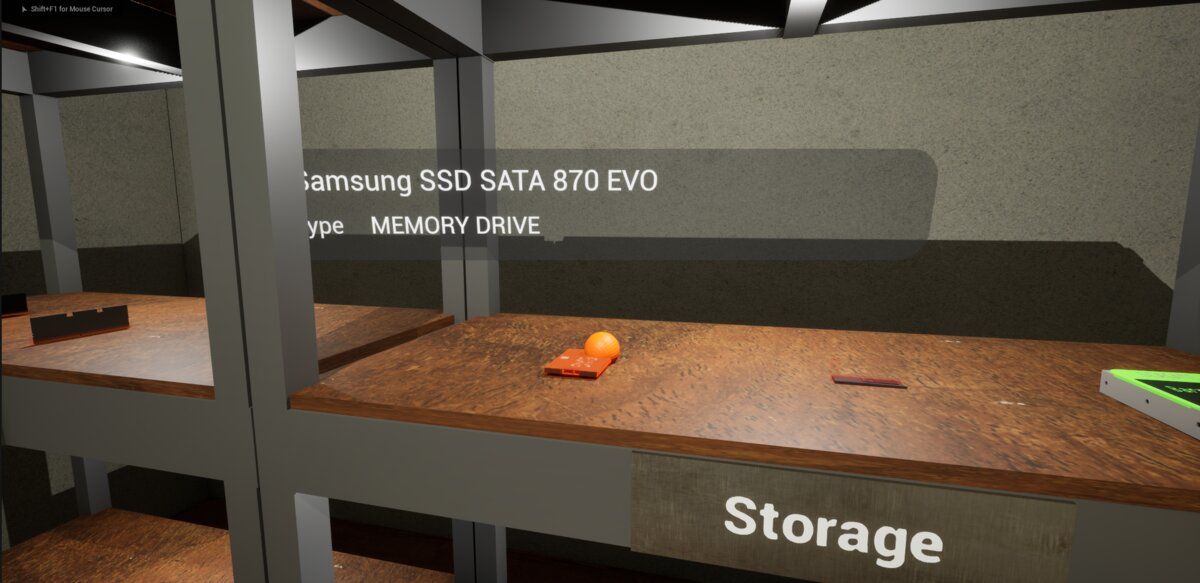
\includegraphics[width=0.958\textwidth]{Images/FinalAssembly140-optimized-hard.jpg}
	\caption{Despite knowing the case is not compatible, the user picks an SSD to install in the case.}
	\label{fig:FinalAssembly140}
\end{figure}

\begin{figure}[H]
	\centering
	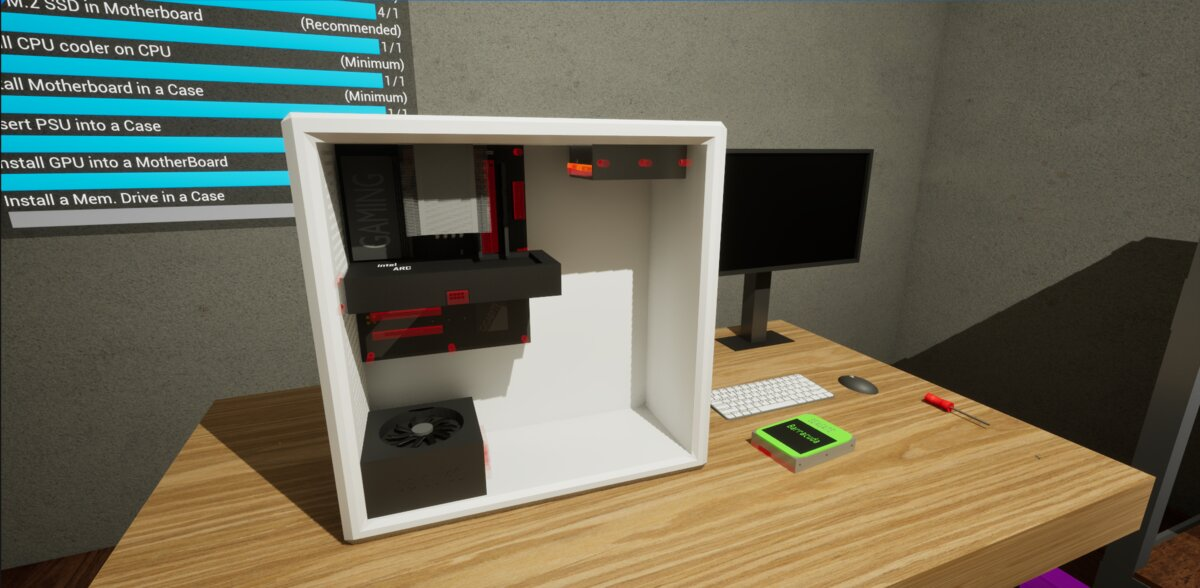
\includegraphics[width=0.958\textwidth]{Images/FinalAssembly150-optimized-hard.jpg}
	\caption{Despite lining it up correctly, the SSD does not highlight as possible to be connected with the case, indicating incompatibility.}
	\label{fig:FinalAssembly150}
\end{figure}

% \begin{figure}[H]
% 	\centering
% 	\subfigure[]{
% 		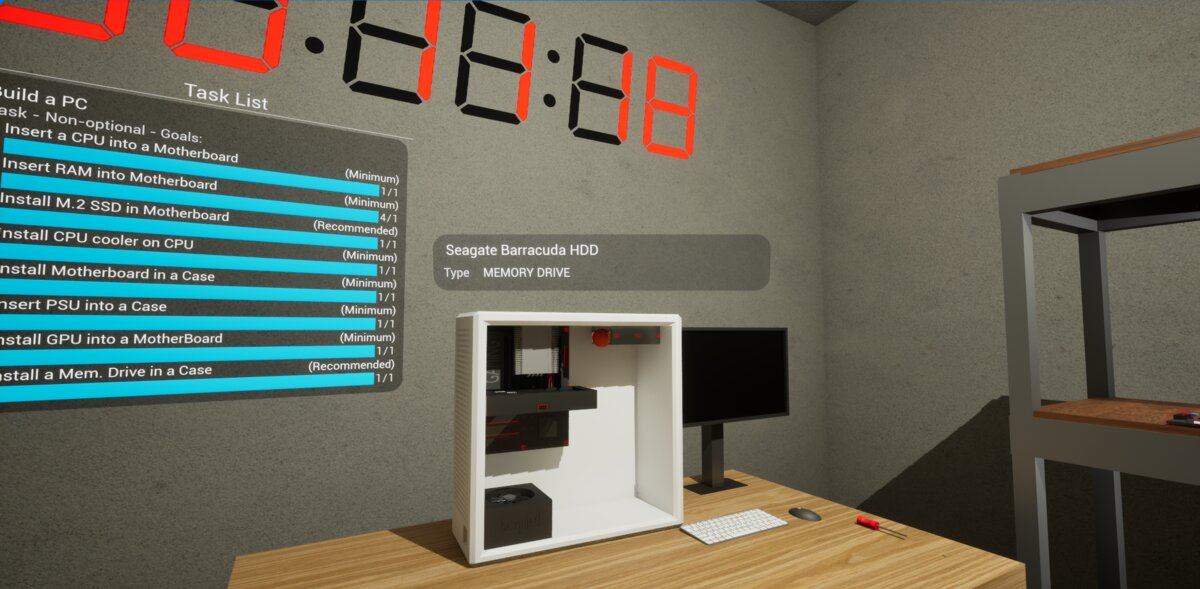
\includegraphics[width=0.45\textwidth]{Images/FinalAssembly160-optimized-hard.jpg}
% 		\label{fig:FinalAssembly160}
% 	}%
% 	\hfil
% 	\subfigure[]{
% 		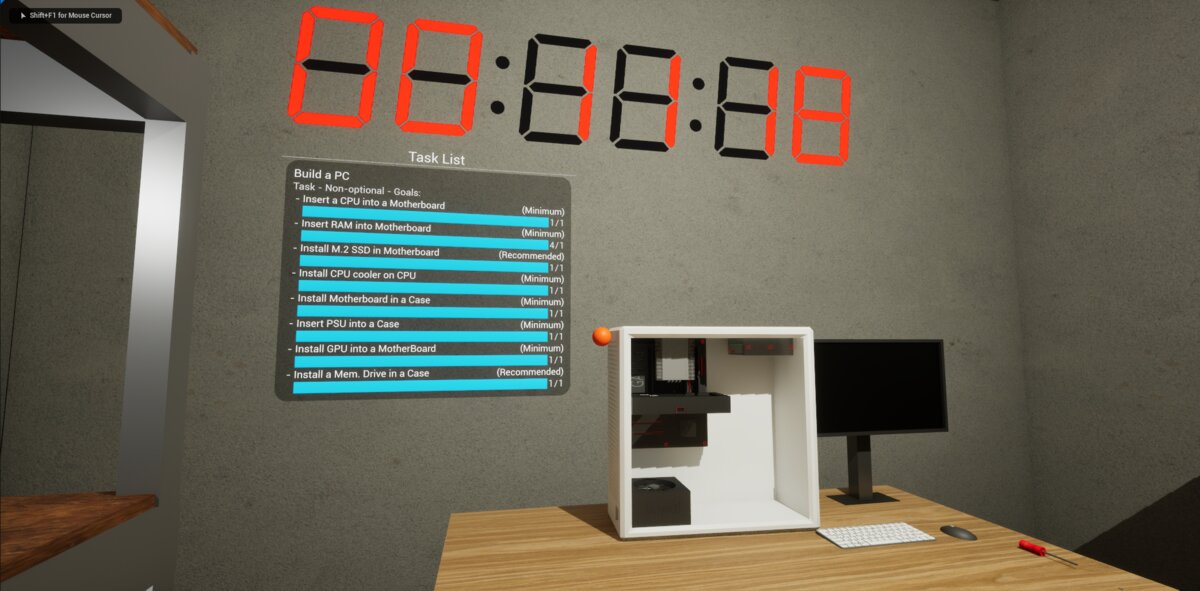
\includegraphics[width=0.45\textwidth]{Images/FinalAssembly170-optimized-hard.jpg}
% 		\label{fig:FinalAssembly170}
% 	}
% 	\caption{Finishing the build: (a) The hard drive has been installed in the case. (b) With this, the assembly has concluded - all the tasks are done, and the clock has stopped.}
%     \label{fig:FinalAssembly160-170}
% \end{figure}

\begin{figure}[H]
	\centering
	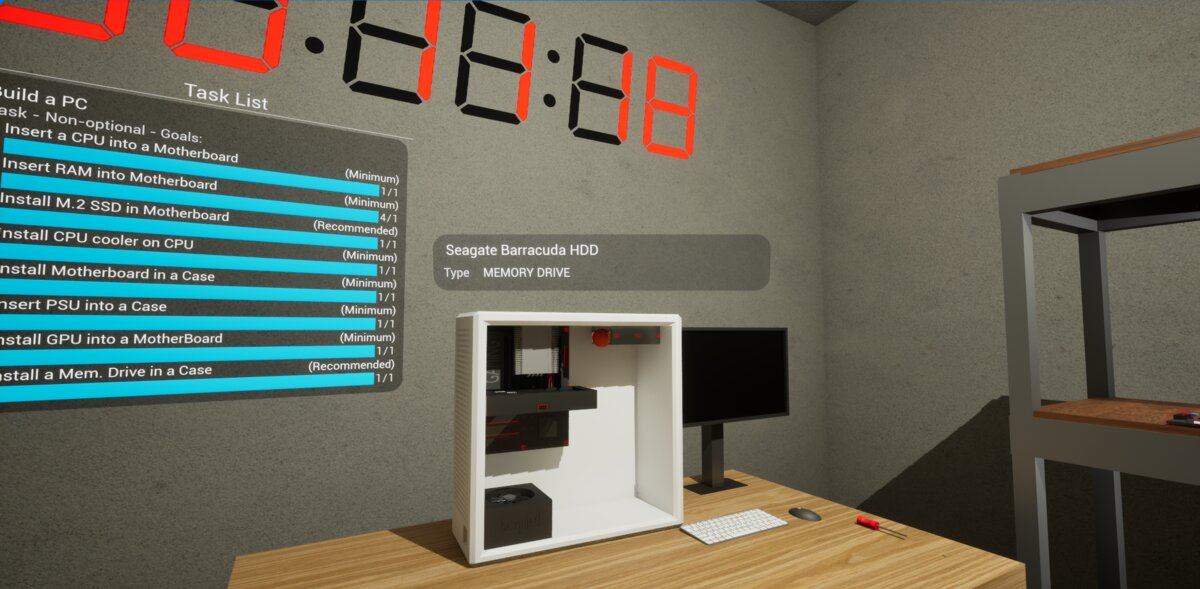
\includegraphics[width=0.958\textwidth]{Images/FinalAssembly160-optimized-hard.jpg}
	\caption{The hard drive has been installed in the case.}
	\label{fig:FinalAssembly160}
\end{figure}

\begin{figure}[H]
	\centering
	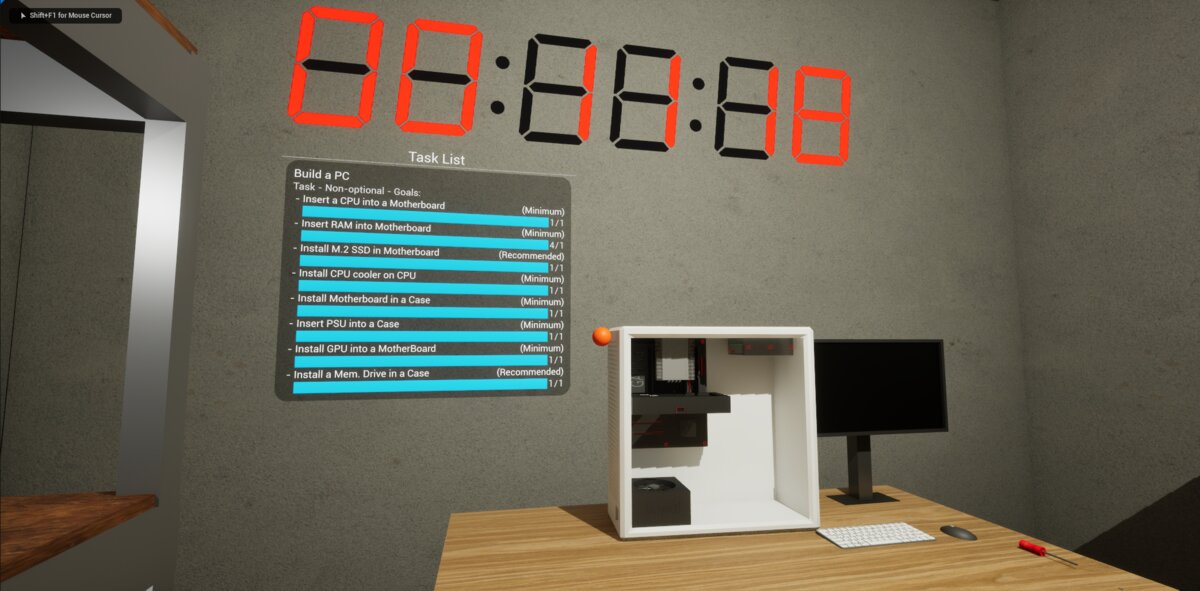
\includegraphics[width=1.0\textwidth]{Images/FinalAssembly170-optimized-hard.jpg}
	\caption{With this, the assembly has concluded - all the tasks are done, and the clock has stopped.}
	\label{fig:FinalAssembly170}
\end{figure}